\chapter{Determining Structural Correspondences}\label{background2}
In order to construct structural generalizations describing the commonalities and differences between logged methods (LMs), we need to find structural correspondences between their ASTs. Therefore, we first need a concrete framework for constructing and manipulating ASTs. The Eclipse integrated development environment provides such a framework in its Java Development Tools (JDT) component. The details of our implementation will depend on certain details of Eclipse JDT, so we describe those in Section~\ref{JDT}.
%constructing?

The correspondence tool, is an Eclipse plug-in I used to determine structural correspondences between nodes in the tree structures. As AST structure does not allows the insertion of variables, I first created an extended form of AST, called AUAST (Anti-unifier AST) that addresses this issue (see Section~\ref{AUAST}), and then applied Jigsaw \cite{2008:fse:cottrell} on these structures, which is a framework exists for determining structural correspondences and measuring similarity between the nodes involved in each correspondence (described in Section~\ref{Jigsaw}). We build atop that work in order to create our anti-unifiers. In addition, an experimental study was conducted to validate the effectiveness of Jigsaw for our application.
%we or I???
% and a comparison of our tool with Jigsaw (Section~\ref{comparison-Jigsaw}).


\section{The Correspondence tool} \label{correspondenceTool}
The correspondence tool is an Eclipse plug-in that inputs ASTs of LJMs of a Java program, creates an extended form of AST structure, called AUAST, to allow the application of HOAUMT, and determines structural correspondences between AUASTs using the Jigsaw framework in a pairwise manner. This process will be described in the following sections.

\subsection{Constructing the AUAST} \label{AUAST}
\RW{This is a concrete implementation, not a generic idea, at least not the way it is described. I strongly suggest that you give a generic description of your assumptions about ASTs then relate AUASTs to those, then talk about implementation details.}
\NZ{I explained it as a part of the implementation of my tool.}

%An anti-unifier AST (AUAST) is an extended form of AST that allows the insertion of variables in place of any node in the tree structure, including both subtrees and leaves, to indicate variations between original structures. The AUAST addresses the limitations of AST to construct an anti-unifier by adding the following structural properties:


The goal of this phase is to construct an extended form of AST structure that would allow the creation of an anti-unified structure. As described in Section~\ref{HOAUMT}, an anti-unified structure utilizes variables that must be substituted with proper substructures to regain original structures. However, an AST structure does not contain any variables, and therefore an extended form of it is required, namely the AUAST (anti-unifier AST), that would allow the insertion of variables in place of any node in the tree structure, including both subtrees and leaves, to indicate variations between the original structures. The AUAST structure addresses the limitations of AST to construct an anti-unifier by adding the following structural properties:
%namely?

\begin{itemize} [leftmargin=.5in]
\item \textit{Simple structural variable Properties}: an extension of simple structural properties referring to two simple values to allow the insertion of variables in place of leaves.
\end{itemize}
\begin{itemize} [leftmargin=.5in]
\item \textit{Child structural variable properties}: an extension of child structural properties referring to two child AST nodes to allow the insertion of variables in place of subtrees.
\end{itemize}

%%???

To provide an example to demonstrate this structure, the anti-unified AUAST constructed from the AUASTs of logging calls in Figures~\ref{ch3-ex1} and~\ref{ch3-ex2} is depicted in Figure~\ref{fig:logging-anti}. The structural variables $X$ and $Y$ are used to indicate the structural variations, where the $X$ structural variable refers to two simple values and the $Y$ structural variable refers to two child nodes. The substitutions are defined in Equations~\ref{eq:theta1} and~\ref{eq:theta2}.

\begin{align}
\Theta_1 = (X \rightarrow \text{ \textsf{\small WARNING}}, Y \rightarrow \text{ \textit{additionExpression}(}\hspace*{3cm}\nonumber\\
\text{\textit{methodCall}(\textit{simpleName}(\textsf{\small getClassName}), \textit{arguments}()),}\nonumber\\
\text{\textit{stringLiteral}(\textsf{\small "should extend ..."}),}\hspace*{4cm}\nonumber\\
\text{\textit{methodCall}(\textit{simpleName}(\textsf{\small handleMessage}), \textit{arguments}()))})\hspace*{-1em}\label{eq:theta1}
\end{align}

\begin{align}
\Theta_2 = (X \rightarrow \text{ \textsf{\small ERROR}}, Y \rightarrow \text{ \textit{additionExpression}(}\hspace*{3cm}\nonumber\\
\text{\textit{stringLiteral}(\textsf{\small "Unknown action: "})},\nonumber\\
\text{ \textit{simpleName}(\textsf{\small actionName}))})\hspace*{-1cm}\label{eq:theta2}
\end{align}

%\item it can be mapped to our recursive definition of a term, where AST nodes and simple values may be viewed as function-symbols and constants, respectively

\begin{figure}[p]
\begin{small}
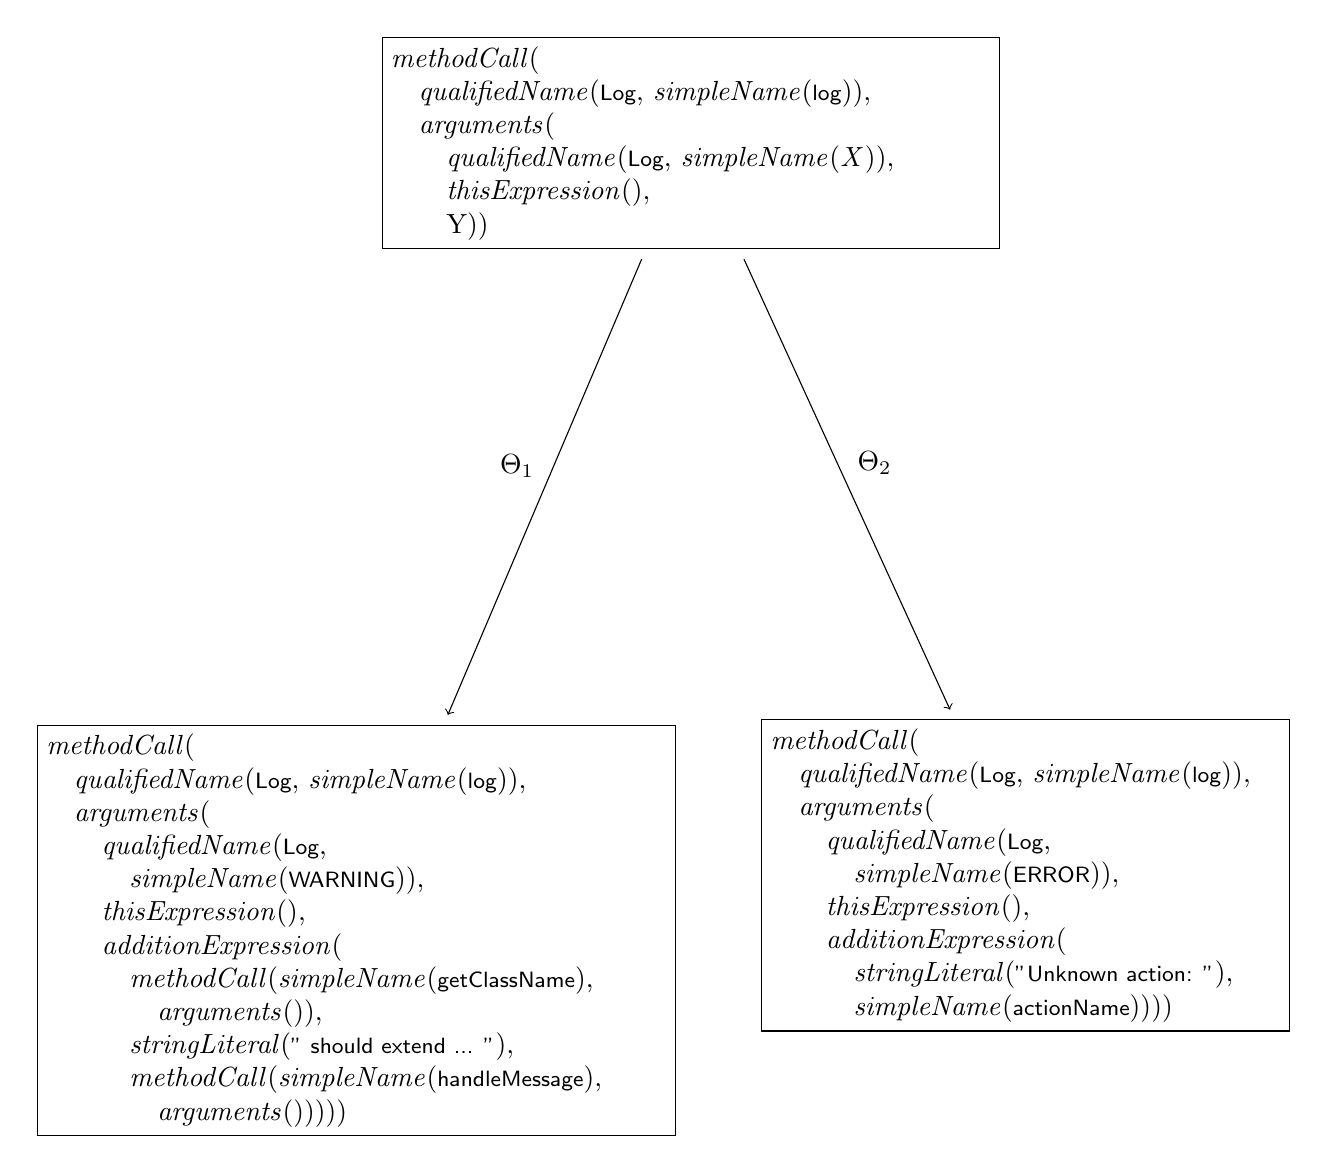
\begin{tikzpicture}
\node(a) at (4.25,10) {%
\fbox{\parbox[b][][b]{3in}{%
\text{\textit{methodCall}(}\\
\text{\hspace*{1em}\textit{qualifiedName}(\textsf{\footnotesize Log}, \textit{simpleName}(\textsf{\footnotesize log})),}\\
\text{\hspace*{1em}\textit{arguments}(}\\
\text{\hspace*{2em}\textit{qualifiedName}(\textsf{\footnotesize Log}, \textit{simpleName}(\textit{X})),}\\
\text{\hspace*{2em}\textit{thisExpression}(),}\\
\text{\hspace*{2em}Y))}}}%
};
\node(b) at (0,0) {%
\fbox{\parbox[t][][b]{3.1in}{%
\text{\textit{methodCall}(}\\
\text{\hspace*{1em}\textit{qualifiedName}(\textsf{\footnotesize Log}, \textit{simpleName}(\textsf{\footnotesize log})),}\\
\text{\hspace*{1em}\textit{arguments}(}\\
\text{\hspace*{2em}\textit{qualifiedName}(\textsf{\footnotesize Log},}\\ \text{\hspace*{3em}\mbox{\textit{simpleName}(\textsf{\footnotesize WARNING})}),}\\
\text{\hspace*{2em}\textit{thisExpression}(),}\\
\text{\hspace*{2em}\textit{additionExpression}(}\\
\text{\hspace*{3em}\textit{methodCall}(\textit{simpleName}(\textsf{\footnotesize getClassName}),}\\ \text{\hspace*{4em}\textit{arguments}()),}\\
\text{\hspace*{3em}\textit{stringLiteral}(\textsf{\footnotesize " should extend ... "}),}\\
\text{\hspace*{3em}\textit{methodCall}(\textit{simpleName}(\textsf{\footnotesize handleMessage}),}\\ \text{\hspace*{4em}\textit{arguments}()))))}}}%
};
\node(c) at (8.5,0.7) {%
\fbox{\parbox[t][][b]{2.55in}{%
\text{\textit{methodCall}(}\\
\text{\hspace*{1em}\textit{qualifiedName}(\textsf{\footnotesize Log}, \textit{simpleName}(\textsf{\footnotesize log})),}\\
\text{\hspace*{1em}\textit{arguments}(}\\
\text{\hspace*{2em}\textit{qualifiedName}(\textsf{\footnotesize Log},}\\ \text{\hspace*{3em}\mbox{\textit{simpleName}(\textsf{\footnotesize ERROR})}),}\\
\text{\hspace*{2em}\textit{thisExpression}(),}\\
\text{\hspace*{2em}\textit{additionExpression}(}\\
\text{\hspace*{3em}\textit{stringLiteral}(\textsf{\footnotesize "Unknown action: "}),}\\
\text{\hspace*{3em}\textit{simpleName}(\textsf{\footnotesize actionName}))))}}}%
};

\draw[->](a) -- (b) node[pos=0.5,above]{$\Theta_1\qquad$};
\draw[->](a) -- (c) node[pos=0.5,above]{$\qquad\Theta_2$};
\end{tikzpicture}
\end{small}
\caption{Anti-unification of the AUASTs of the logging calls in Examples 1 and 2.\label{fig:logging-anti}}
\end{figure}
%The AUASTs of log Method Invocation nodes from the Java classes in Figure~\ref{ch3-ex1} and Figure~\ref{ch3-ex2}.




%\begin{align}
%\Theta_1 = (W &\rightarrow \text{ \textsf{\small WARNING}},\nonumber\\
%X &\rightarrow \text{ \textit{methodCall}(\textit{simpleName}(\textsf{\small getClassName}), \textit{arguments}())},\nonumber\\
%Y &\rightarrow \text{ \textsf{\small "should extend EditPlugin not EBPlugin since it has an empty "}},\nonumber\\
%Z &\rightarrow \text{ \textit{methodCall}(\textit{simpleName}(\textsf{\small handleMessage}), \textit{arguments}())})\label{eq:theta1}\\
%\Theta_2 = (W &\rightarrow \text{ \textsf{\small ERROR}},\nonumber\\
%X &\rightarrow \text{ \NIL{}},\nonumber\\
%Y &\rightarrow \text{ \textsf{\small "Unknown action: "}},\nonumber\\
%Z &\rightarrow \text{ \textit{simpleName}(\textsf{\small actionName})})\label{eq:theta2}
%\end{align}
%
%%\item it can be mapped to our recursive definition of a term, where AST nodes and simple values may be viewed as function-symbols and constants, respectively
%
%\begin{figure}[p]
%\begin{small}
%\begin{tikzpicture}
%\node(a) at (4.25,10) {%
%\fbox{\parbox[b][][b]{3in}{%
%\text{\textit{methodCall}(}\\
%\text{\hspace*{1em}\textit{qualifiedName}(\textsf{\footnotesize Log}, \textit{simpleName}(\textsf{\footnotesize log})),}\\
%\text{\hspace*{1em}\textit{arguments}(}\\
%\text{\hspace*{2em}\textit{qualifiedName}(\textsf{\footnotesize Log}, \textit{simpleName}(\textit{W})),}\\
%\text{\hspace*{2em}\textit{thisExpression}(),}\\
%\text{\hspace*{2em}\textit{additionExpression}(\textit{X}, \textit{stringLiteral}(\textit{Y}), \textit{Z})))}}}%
%};
%\node(b) at (0,0) {%
%\fbox{\parbox[t][][b]{3.1in}{%
%\text{\textit{methodCall}(}\\
%\text{\hspace*{1em}\textit{qualifiedName}(\textsf{\footnotesize Log}, \textit{simpleName}(\textsf{\footnotesize log})),}\\
%\text{\hspace*{1em}\textit{arguments}(}\\
%\text{\hspace*{2em}\textit{qualifiedName}(\textsf{\footnotesize Log},}\\ \text{\hspace*{3em}\mbox{\textit{simpleName}(\textsf{\footnotesize WARNING})}),}\\
%\text{\hspace*{2em}\textit{thisExpression}(),}\\
%\text{\hspace*{2em}\textit{additionExpression}(}\\
%\text{\hspace*{3em}\textit{methodCall}(\textit{simpleName}(\textsf{\footnotesize getClassName}),}\\ \text{\hspace*{4em}\textit{arguments}()),}\\
%\text{\hspace*{3em}\textit{stringLiteral}(\textsf{\footnotesize " should extend ... "}),}\\
%\text{\hspace*{3em}\textit{methodCall}(\textit{simpleName}(\textsf{\footnotesize handleMessage}),}\\ \text{\hspace*{4em}\textit{arguments}()))))}}}%
%};
%\node(c) at (8.5,0.7) {%
%\fbox{\parbox[t][][b]{2.55in}{%
%\text{\textit{methodCall}(}\\
%\text{\hspace*{1em}\textit{qualifiedName}(\textsf{\footnotesize Log}, \textit{simpleName}(\textsf{\footnotesize log})),}\\
%\text{\hspace*{1em}\textit{arguments}(}\\
%\text{\hspace*{2em}\textit{qualifiedName}(\textsf{\footnotesize Log},}\\ \text{\hspace*{3em}\mbox{\textit{simpleName}(\textsf{\footnotesize ERROR})}),}\\
%\text{\hspace*{2em}\textit{thisExpression}(),}\\
%\text{\hspace*{2em}\textit{additionExpression}(}\\
%\text{\hspace*{3em}\textit{stringLiteral}(\textsf{\footnotesize "Unknown action: "}),}\\
%\text{\hspace*{3em}\textit{simpleName}(\textsf{\footnotesize actionName}))))}}}%
%};
%
%\draw[->](a) -- (b) node[pos=0.5,above]{$\Theta_1\qquad$};
%\draw[->](a) -- (c) node[pos=0.5,above]{$\qquad\Theta_2$};
%\end{tikzpicture}
%\end{small}
%\caption{The anti-unification of the AUASTs of the logging calls in Examples 1 and 2.\label{fig:logging-anti}}
%\end{figure}
%%The AUASTs of log Method Invocation nodes from the Java classes in Figure~\ref{ch3-ex1} and Figure~\ref{ch3-ex2}.

%Applying higher-order anti-unification on AUAST structures could help to construct a structural generalization by maintaining the common pieces and abstracting the differences away using variables. However, it is not comprehensive enough to solve our problem as it does not consider background knowledge about AST structures, such as syntactically different but semantically relevant structures, missing structures, and different ordering of arguments. In the following section, we will look at an extension of anti-unification, higher-order anti-unification modulo theories, and how it can sufficiently address the limitations of anti-unification in our context.

%We provide an example to demonstrate the AUAST structure, which is limited to log method invocation subtrees of the sample Java classes shown in Figure~\ref{fig:constructAUast}. The log method invocation nodes both contains \texttt{EXPRESSION}, \texttt{ARGUEMENTS}, and \texttt{NAME} structural properties which are made up of \texttt{\bold{Log}}, \texttt{\bold{Log}}, \texttt{\bold{WARNING}} simple values for the AUAST1 and  \texttt{\bold{Log}}, \texttt{\bold{Log}}, \texttt{\bold{ERROR}} simple values for the AUAST2, respectively. The structural representation of the AUASTs as defined in Section~\ref{back-str} is \texttt{EXPRESSION[EXPRESSION[IDENTIFIER[\bold{Log}]], ARGUMENTS[QUALIFIER[IDENT\\IFIER[\bold{Log}]], NAME[IDENTIFIER[\bold{WARNING}]]}for the AUAST1 and \texttt{EXPRESSION[EX\\PRESSION[IDENTIFIER[\bold{Log}]], ARGUMENTS[QUALIFIER[IDENTIFIER[\bold{Log}]], \\NAME[IDENTIFIER[\bold{ERROR}]]} for the AUAST2, where the words capitalized represents subtrees and the words shown in bold represents leaves of the tree structure.

%\begin{figure} [H]
 % \centering\includegraphics [width = \textwidth, height = 0.4\textheight]
 % {Drawing4/structure1.pdf}
 % \caption{The AUASTs of log Method Invocation nodes from the Java classes in Figure~\ref{ch3-ex1} and Figure~\ref{ch3-ex2}.}
 % \label{fig:constructAUast}
%\end{figure}


\subsection{Determining structural correspondences}\label{Jigsaw_usage}

Our correspondence tool applies a part of the implementation of Jigsaw to identify structural correspondences between AUASTs and reuses the Jigsaw similarity function to measure the similarity between nodes involved in each correspondence connection. However, the Jigsaw tool does not suffice to construct an anti-unifier that is the best fit to our application, as the problem of this study is different. In addition, the Jigsaw similarity function does not measure the similarity of two LJMs with a focus on logging calls, which is needed in our context. To address these issues, we should develop a greedy selection algorithm to approximate the best anti-unifier for our problem by determining the best correspondence for each node. In the following chapter, we will discuss our approach to construct structural generalization and our implementation by means of the higher-order anti-unification modulo theories and the Jigsaw framework.
%to construct structural generalizations?

\section{An Assessment of the Correspondence tool}\label{jigsaw-assessment}

\RW{Describe here the procedure you used to select the examples, etc., how you tested Jigsaw, and what your findings were. At some point, you complained that Cottrell had not done something right ... do you have any evidence to demonstrate it?  How does this affect your work?  Such points can go in a discussion section towards the end of this chapter if they don't fit otherwise.  Full details of examples can go in an appendix; here, just describe enough so people can get the point.}

\NZ{I think this experiment is not much about evaluating Jigsaw (The evaluation was conducted by Cottrell), but it is more about understanding what Jigsaw does and how to use it for my application . What I have mentioned was about detecting relevance links which is not related to my work. During my development, I added some statements to Jigsaw for the cases that was not covered in his work completely (e.g, Jigsaw did not detect the correspondence between inner type declarations of two nested type declarations when comparing the two upper type declarations }

%chapter{Experimental Studies}  \label{studies}
%To evaluate our approach, we have implemented a tool, and conducted three empirical studies on a set of LJMs extracted from a real-world software system. In this section, we describe our experimental setup, present our studies, and discuss the results.

We have conducted an experiment on a set of LJMs extracted from a real-world software system to assess how Jigsaw could effectively help us determine potential correspondences between AST nodes and measure similarity between them.
We implemented a plug-in to the Eclipse integrated development environment (IDE), which uses the \name{JDT} framework to extract ASTs of a pair of LJMs and applies the \name{Jigsaw} framework to generate correspondence connections between AST nodes.

%the correspondence tool as
%\subsubsection{Experimental Setup}  \label{study1_setup}
\subsection{Setup}  \label{study1_setup}
%Our tool is a plug-in to the Eclipse integrated development environment (IDE) that implements our algorithm. The tool consists of three main components: a correspondence tool, an antiunifier-building tool, and a clustering tool. The correspondence tool inputs a pair of LJMs, uses the Jigsaw framework to determine potential correspondences between their AST nodes, and outputs the generated CASTs and the Jigsaw similarity between them. The antiunifier-building tool inputs a pair of LJMs, applies our anti-unification algorithm to construct an anti-unifier with a special attention to logging calls, and outputs the detailed view of anti-unifier and similarity measure (as described in Section~\ref{meth-antiUnifier}). The clustering tool inputs a set of LJMs, applies a hierarchical clustering algorithm to classify them based on the similarity measurement, and outputs the detailed view of the generated anti-unifier for each cluster (as described in Section~\ref{meth-clustering}).
% figure of architecture?

As a subject for our study, we used \name{jEdit}, a programmer’s text editor tool written in Java programming language. We chose this subject because it is a real program that has been used constantly by many developers, and it employs real usage of logging calls. Our tool extracts all LJMs within the source code of this program. However, a subset of them was selected containing 9 LJMs that showed varying levels of similarity on manual examination, and it has been used as a test suite throughout this study (see Table~\ref{table:ljms}). The org.gjt.sp.jedit.EditBus.send(...) method contains two logging calls. To handle this case we split it into two cases: case 3 contained the first logging call while the second one was removed; case 4 contained only the second logging call. We will describe our approach for LJMs containing multiple logging calls in details in Section~\ref{meth-multipleLogs}. The last three LJMs were manually modified by adding some statements for the sake of dealing with important cases that we otherwise would have missed testing. Case 8 simulates the addition of an \code{if- }statement that formed a nested \code{if- }statement enclosing a logging call. Cases 9 and 10 simulate the addition of statements to improve the test coverage.


\begin{figure} [H]
  \centering
  \begin{tabular}{|c|l|c|}
    \hline
    Case & Logged Java methods & Size(LOC)\\
    \hline
    1& org.gjt.sp.jedit.PluginJAR.generateCache() &104\\
   \hline
    2& org.gjt.sp.jedit.MiscUtilities.isSupportedEncoding(...) &9\\
   \hline
    3& org.gjt.sp.jedit.EditBus.send(...) &14\\
   \hline
    4& org.gjt.sp.jedit.EditBus.send(...)* &14\\
   \hline
    5& org.gjt.sp.jedit.EditAction.Wrapper.actionPerformed(...) &5\\
   \hline
    6& org.gjt.sp.jedit.EBPlugin.handleMessage(...) &6\\
   \hline
    7& org.gjt.sp.jedit.BufferHistory.RecentHandler.doctypeDecl(...) &3\\
   \hline
    8& org.gjt.sp.jedit.JARClassLoader.loadClass(...) &32\\
   \hline
    9& org.gjt.sp.jedit.io.VFS.DirectoryEntry.RootsEntry.rootEntry(...) &36\\
   \hline
    10& org.gjt.sp.jedit.ServiceManager.loadServices(...) &20\\
    \hline
  \end{tabular}
  \caption[Logged Java methods used as our test suite.]{Logged Java methods used as our test suite; all are contained in the \protect\name{org.gjt.sp.jedit} package.}
  \label{table:ljms}
\end{figure}


%\subsubsection{Setup}  \label{study1-setup}
Our tool was used to compare LJMs of our test suite in a pairwise manner (55 test cases in total, including self-comparisons) and to produce the CASTs of each pair. The Jigsaw similarity was also measured for each of these test cases.
We examined the generated CASTs of these test cases and selected a subset of 4 cases with various levels of correspondences as depicted in the Table~\ref{jigsaw_4_test_cases}. Case 1 contains the comparison of a Java element with itself. Case 2 contains the comparison of two Java elements that are both syntactically and semantically dissimilar.  Case 3 contains the correspondence between two Java elements that are syntactically dissimilar but are semantically relevant. Case 4 contains the comparison of a logging call with another Java element that is not logging call but is syntactically relevant.

\subsection{Results}  \label{study1-results}
The results of the pairwise comparison between LJMs of the test suite is visualized in Figure~\ref{fig:jigsaw_graph}. As it is shown, the Jigsaw similarity for all self-comparisons is 1, while  the level of Jigsaw similarity is different for pairs containing distinct LJMs as our manual examination.

\begin{figure} [H]
  \centering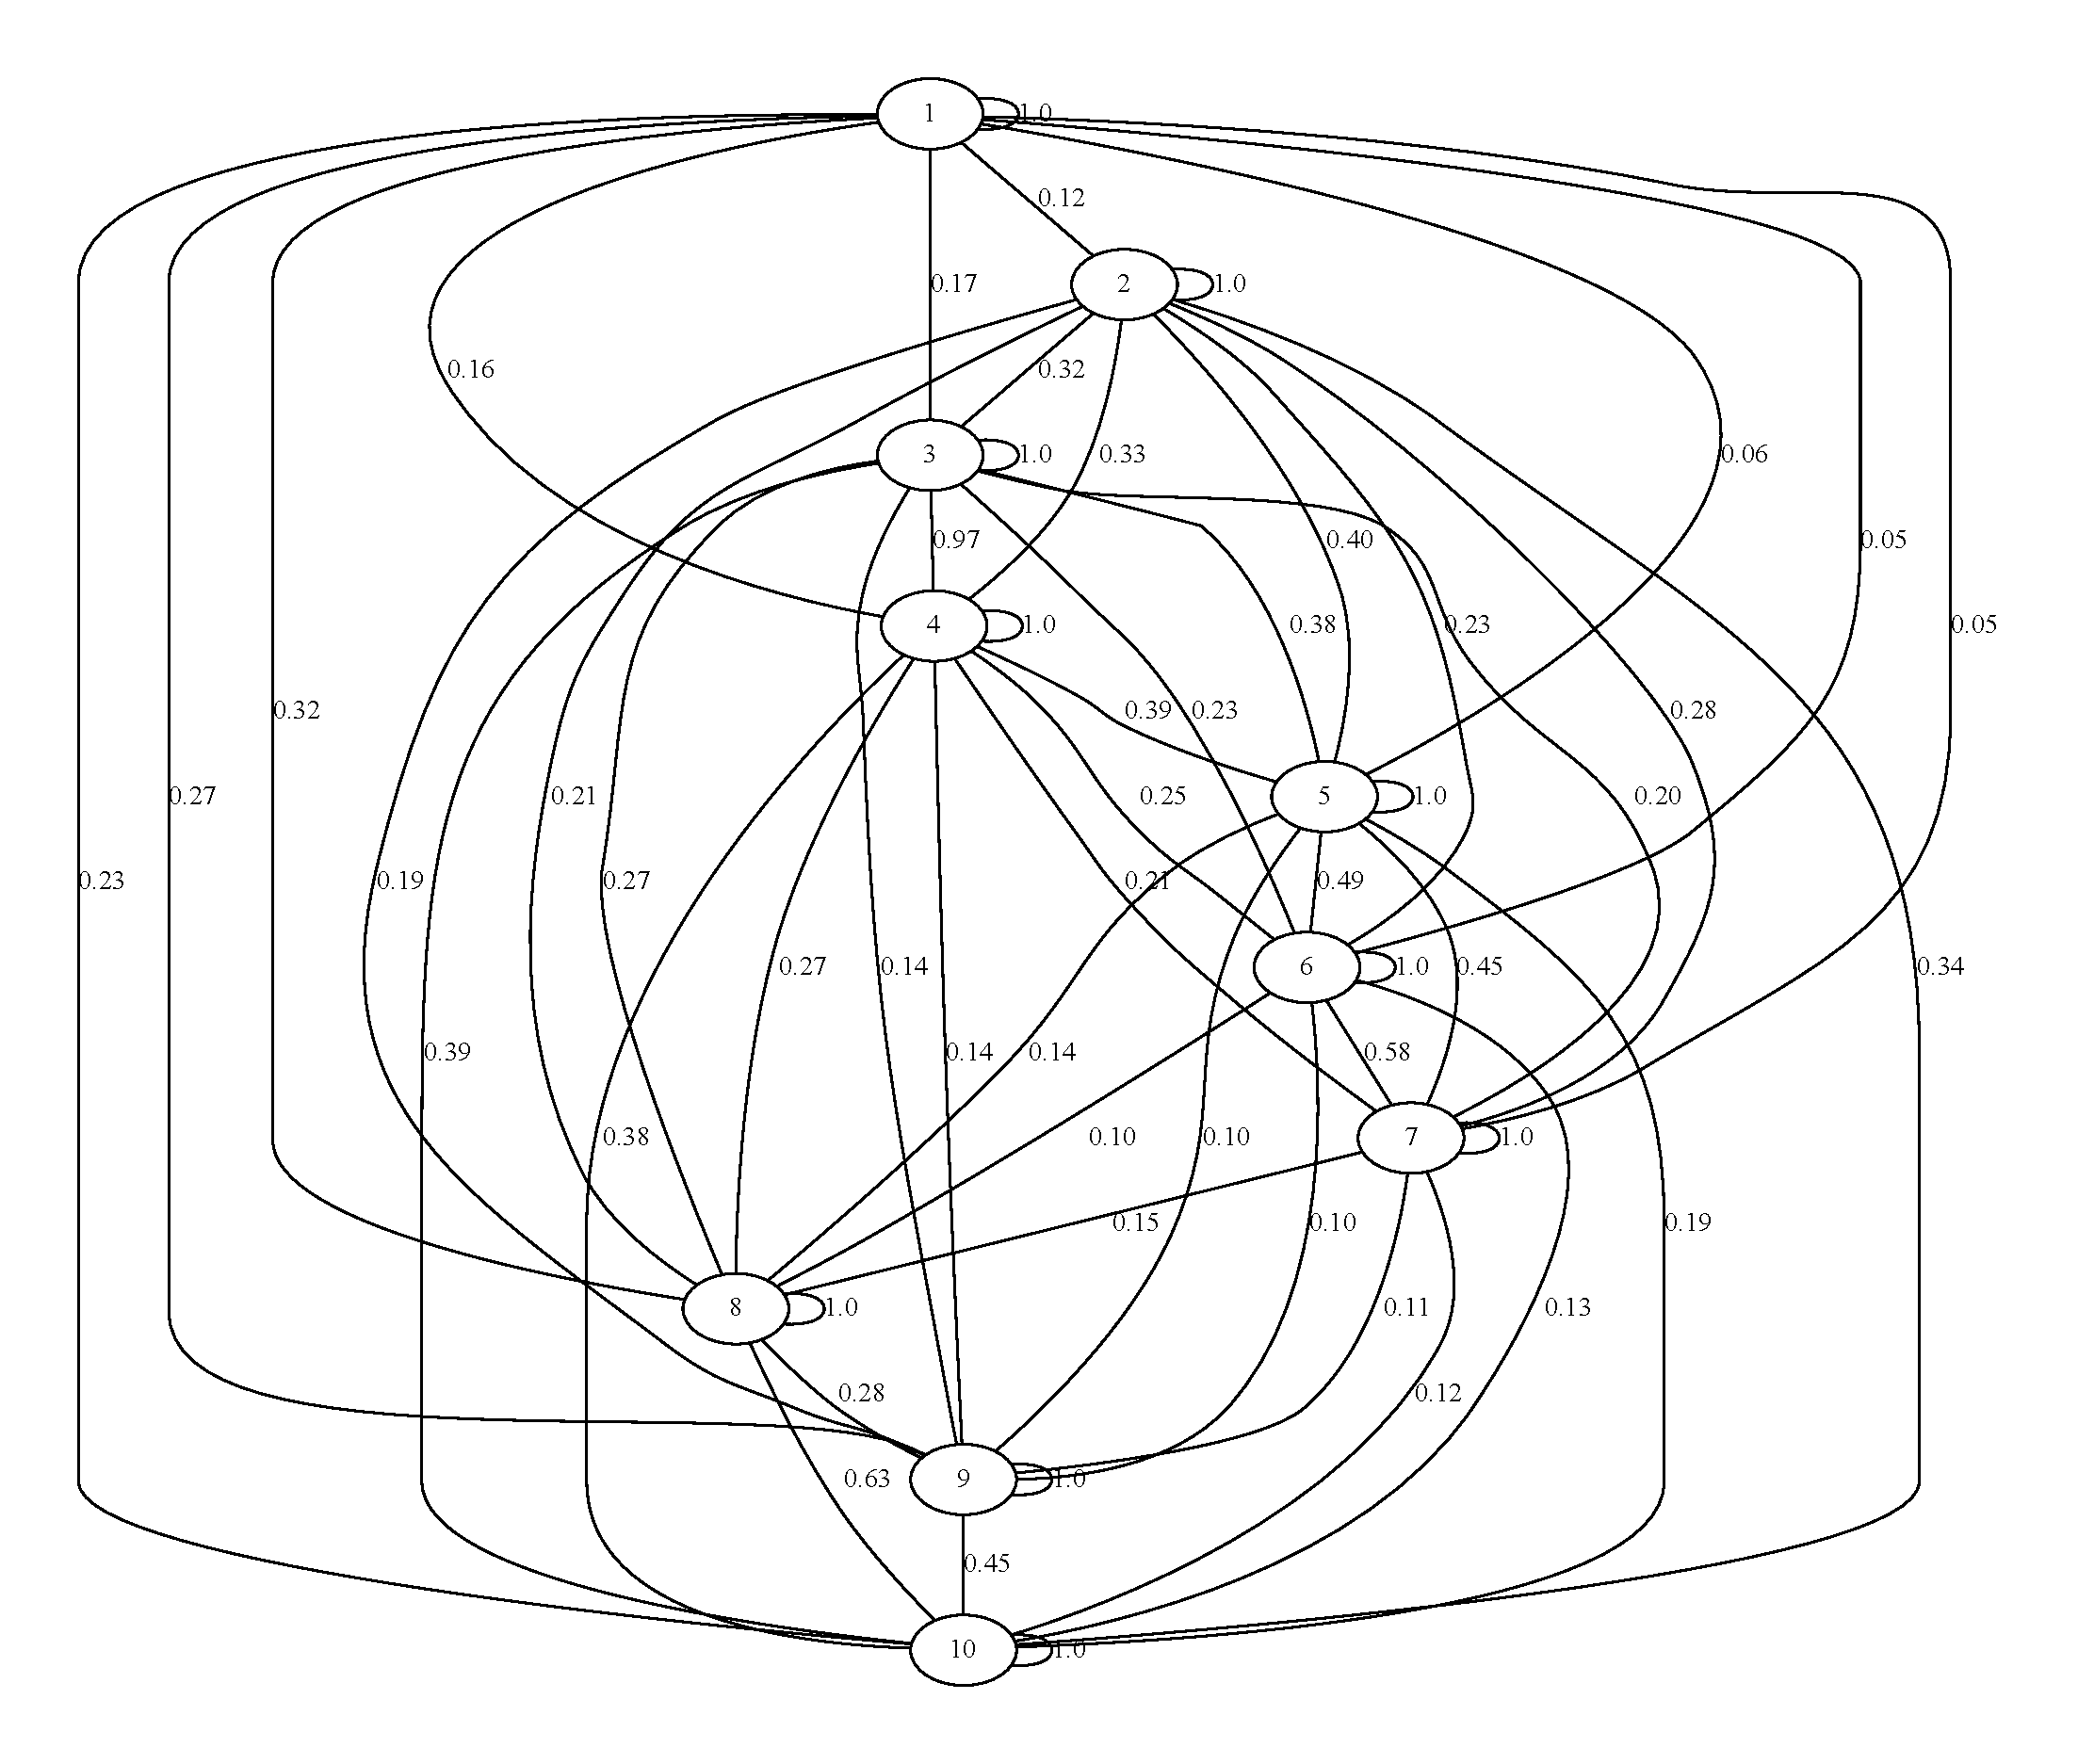
\includegraphics [width = \textwidth]{graphviz/jigsaw.pdf}
  \caption{A similarity graph representing pairwise Jigsaw similarities between LJMs shown in Table~\ref{table:ljms}.}
  \label{fig:jigsaw_graph}
\end{figure}


The analysis of the 4 test cases is shown in Table~\ref{jigsaw_4_test_cases}. Test Case 1 shows that a Java element that is compared with itself has a Jigsaw similarity of 1. Test Case 2 indicates that no correspondence connection is created when a Java element is compared with another Java element that is utterly dissimilar. Test Case 3 indicates that the similarity between a \code{for-} statement and a \code{while-} statement is non-zero, and that Jigsaw is able to detect semantic correspondences between Java elements. Test Case 4 shows that a logging call has non-zero similarity with another Java element that is not a logging call but is syntactically relevant. This case will be handled via the removal of this kind of correspondence connection, as will be described in Section~\ref{meth-constraints}.

\begin{figure}
  \centering
  \begin{tabular}{|c|l|c|}
    \hline
    \shortstack{Test\\case} & Java source code fragment & \shortstack{Jigsaw\\similarity}\\
    \hline

    \multirow{2}{*}{{1}}&Log.log(Log.WARNING,this,"Unknown action: " + actionName);& \multirow{2}{*}{1}\\
    \cline{2-2}
                         &Log.log(Log.WARNING,this,"Unknown action: " + actionName);\\
    \hline

       \multirow{2}{*}{2}&return entry& \multirow{2}{*}{\shortstack{No\\correspondence \\connection}}\\
    \cline{2-2}
       &int i=0;\\
    \hline


 \multirow{2}{*}{3}&
 for (int i=0; i < comps.length; i++) {...} \\


    \cline{2-2}
      &
while (entries.hasMoreElements())  { ...}
      \\
    \hline

    \multirow{2}{*}{4}&Log.log(Log.WARNING,this,"Unknown action: " + actionName);& \multirow{2}{*}{0.33}\\
    \cline{2-2}
      &EditBus.removeFromBus(this);\\
    \hline

  \end{tabular}
  \caption{Results from examining the Jigsaw similarity for 4 sample Java source code fragment pairs.}
  \label{jigsaw_4_test_cases}
\end{figure}

%\section{Comparison with the Jigsaw tool}  \label{comparison-Jigsaw}



\section{Summary}  \label{summary}
We described Eclipse JDT as a concrete framework that can be used  to manipulate ASTs of a source code written in the Java programming language. We also introduced Jigsaw, an existing framework for determining structural correspondences between AST nodes and measuring similarity between them. Furthermore, we assess the Jigsaw functionality to address our problem through an empirical study on a set of LJMs selected from a real- world software system.







%In this chapter, we described anti-unification as a technique to construct a common generalization of two given terms. We have also introduced an extended form of anti-unification, which is called higher-order anti-unification modulo theories, where a set of equivalence equations can be applied on higher-order extended structures to incorporate background knowledge. In addition, we provided a brief description of AST that maps Java source code in a tree structure form, and why an extended form of it, named AUAST, is required to create higher-order structures specific to our problem context. Finally, we discuss the Jigsaw framework and how it could assist us in determining the potential structural correspondences. 